%\part{Résumé de thèse}

\selectlanguage{frenchb}
\chapter{Résumé de thèse}

Ce chapitre offre un résumé de la thèse défendue dans ce document. Pour ce faire, une introduction au contexte de ce travail, permettra de mettre en évidence les besoins que la contribution de cette thèse s'est attachée à combler. Puis, la contribution à proprement parlée est décrite et discutée en termes d'adéquation aux besoins. Enfin, une mise en évidence des bénéfices immédiats et de quelques limitations identifiées termine ce chapitre.

\section{Rappel du contexte}

Le vieillissement de la population Européenne a incité la communauté à rechercher des solutions pour accompagner ce changement. Dans ce contexte, plusieurs problèmes doivent être considérés de front. D'abord, le domaine de la santé souffre d'une pénurie de main d'\oe uvre, qui pourrait résulter en une dégradation générale de la qualité des soins. Par ailleurs, les places en centres hospitaliers ou maisons de retraites sont limitées, et pourraient arriver à saturation dans les années à venir. De plus, les séjours hospitaliers coûtent chère, indépendamment de la pathologie, et les aides financières à ce niveau tendent à être limitées.\\
Plusieurs projets ont déjà été lancés pour de tenter de répondre à ces problématiques. Le programme collaboratif Européen {\it Ambient Assisted Living}(AAL) a été créé pour favoriser et financer des projets, ce qui met en évidence l'intérêt de l'Europe pour les avancées dans ce domaine. Le projet {\it Innovation Domicile Autonomie}(IDA), initié par la métropole Rennaise, s'inscrit parfaitement dans ce cadre. Il vise une évaluation de la pertinence d'utiliser des Technologies de l'Information et de la Communication(TIC) pour aider les personnes âgées.\\
Après un état des lieux précis, en termes de besoin des personnes âgées, le projet s'est efforcé de mesurer la pertinence et l'adéquation de différentes technologies industrielles, afin d'assister les personnes dans leurs domiciles. Entre autres, les technologies de la domotique ont été évaluées afin de faire ressortir leurs potentiels apports dans l'accompagnement à domicile. Rapidement, les études ont montré qu'une unique solution ne peut pas être mise en place dans tous les cas. Chaque personne à des exigences et des besoins différents, qui imposent que les solutions soient adaptées à chacun. Aussi, les industriels admettent ici leurs limites, où là fabrication de produits personnalisés pour chaque utilisateur est trop coûteuse.\\

Dans ce domaine, les solutions techniques imaginées ont besoin de systèmes logiciels pour combler le vide, entre les produits finis issus du marché de la domotique, et les solutions personnalisées. Pour remplir leur mission, ces systèmes logiciels doivent satisfaire à plusieurs exigences

\section{Résumé des exigences}
\label{sec:concluRequirementsFr}

{\bf L'interopérabilité} est la première exigence que les systèmes logiciels ont à prendre en compte. En effet, les solutions proposées pour améliorer et favoriser le confort des personnes âgées dans leurs logements, peuvent être composées de multiple produits provenant de divers fabricants. Chaque produit prenant part à la solution, s'atèle à répondre à un des besoins de la personne de la façon la plus précise possible, rapprochant ainsi la proposition globale de la proposition idéale. Cependant, les éléments de la solution doivent aussi être capables de communiquer les uns avec les autres, afin de rendre un service global. Mais la diversité des constructeurs fait de l'interopérabilité des produits un problème de taille.\\
La définition d'une interface de communication, universelle à tous les composants du système, pourrait résoudre ce problème, mais requière une réingénierie de l'ensemble des produits pour les rendre compatibles. En conséquence, aucun produit actuellement sur le marché ne pourrait être utilisé. Tant que les solutions seront non limitées en termes de produits, cette proposition ne sera pas applicable, et l'interopérabilité restera une préoccupation majeure.\\

{\bf L'adaptation et l'évolution} sont aussi des facultés essentielles pour ces systèmes. Les systèmes logiciels travaillant à partir d'objets ou d'équipements, liés à des actions du quotidien, doivent prendre en considération l'environnement dans lequel ils s'exécutent. Ils doivent être capables de s'adapter aux changements pendant leur exécution, afin de maintenir des niveaux de services et de fonctionnalités suffisant. Évidemment, ces adaptations ne doivent pas nécessiter de redémarrage du système, qui rendrait indisponible les fonctions d'alerte ou d'alarme par exemple.\\
Par ailleurs, les besoins, les usages, les protocoles et les technologies évoluent. Des fonctionnalités précédemment installées peuvent devenir inutiles, alors que d'autres deviennent nécessaires. La sécurité, la fiabilité du système, les protocoles peuvent être améliorés et mis à disposition dans de nouvelles versions, qui seront à prendre en compte sans avoir à ré-implémenter le système entier. Enfin, les systèmes logiciels doivent, dans ce domaine, être capable de supporter des évolutions futures non prévues au moment du déploiement, comme l'installation de nouveaux services ou fonctionnalités.\\

{\bf L'ouverture et le contrôle à distance} doivent permettre à des applications tierces, d'accéder aux fonctionnalités ou aux produits disponibles dans le système. En effet, la passerelle de communication avec les réseaux KNX, par exemple, n'admet qu'une seule connexion à la fois. Il est donc nécessaire de rendre les produits et fonctionnalités disponible à d'autres applications, afin de ne pas verrouiller les accès. Par ailleurs, cette ouverture au monde extérieur permet à des applications tierces de se connecter aux produits, et rendre des services à valeur ajoutée, sans avoir besoin de connaître l'organisation interne du système de gestion d'accès aux périphériques. L'ouverture permet donc d'enrichir l'application par des contributions externes apportant des fonctionnalités intelligentes supplémentaires.\\
Les contrôles distants peuvent être nécessaires pour des questions de maintenance, de vérification de l'état de la maison par des professionnels accrédités, ou réaliser des actions à distance pour assister la personne sur des problèmes ponctuels.\\

{\bf La gestion de la variabilité et la distribution} sont des préoccupations liées au fort besoin de personnalisation des solutions, et à la dispersion des déploiements. En effet, l'ensemble des options déployées sur les systèmes à l'échelle d'une ville, peut très vite devenir ingérable. De plus, les évolutions ne sont pas uniformément déployées à l'échelle d'une ville, menant alors à une grande diversité de combinaisons de versions de protocoles, et d'assemblages de produits.\\
Des outils doivent donc être mis à disposition par ces systèmes, pour assister les ingénieurs et techniciens dans la fabrication de solutions. Des outils d'aide à la décision basés sur une liste d'exigences et de produits disponibles pourraient, par exemple, être d'une aide précieuse.\\

{\bf La sûreté et la sécurité} sont des éléments important dans les systèmes domotiques. Ces systèmes se voient confiée la responsabilité de gérer une partie de la maison, afin d'améliorer la vie de ses occupants. Un niveau de service minimum doit être garanti afin que les personnes aidées par ces systèmes ne se retrouvent pas bloqués en cas d'urgence par exemple. Par ailleurs, les accès au système doivent être sécurisés afin d'éviter qu'il soit contrôlé par des personnes non autorisées, mais pas au point d'en faire une contrainte pour les personnels habilités.\\

{\bf L'acceptabilité et l'accessibilité} de ces systèmes par tous les utilisateurs sont des facultés à prendre en compte, particulièrement dans le cadre d'une aide à domicile pour des personnes âgées ou dépendantes. Ces systèmes logiciels sont utilisés à la fois par les aidants à domicile, et par les personnes âgées, et pour ni l'une ni l'autre le système ne doit être perçu comme une contrainte supplémentaire dans leur métier ou leur vie. Enfin, les personnes âgées doivent pouvoir rester maître de leur environnement, et donc, garder la main sur le système et ses actions.\\


\section{Étude des approches existantes}

Parmi l'ensemble des exigences listées dans la section~\ref{sec:concluRequirementsFr}, l'étude des approches existantes ici résumée, s'est concentrée sur les aspects d'interopérabilité, d'adaptation, d'évolution, d'ouverture et de gestion de la variabilité.\\

Les approches s'intéressant à la résolution de problèmes d'interopérabilité, d'adaptation ou de contrôle distant pour différentes applications, sont assez abondantes dans la littérature scientifique.\\
D'une manière générale, les approches s'appuyant sur des architectures à base de services semblent être adaptés pour résoudre des problèmes d'adaptation dynamique et d'interopérabilité, mais manquent clairement de moyens de description de l'architecture du logiciel pendant son exécution. Ils apportent aussi des mécanismes essentiels pour faire face aux apparitions et disparitions de produits, de par le fait qu'un service peut être démarré ou arrêté à tout instant.\\
Les architectures s'appuyant sur le paradigme de composants logiciels, offrent pour leur part un niveau d'abstraction idéal pour représenter les produits domotiques. Cependant, les ports de communication des composants sont souvent définis par l'intermédiaires d'interfaces de programmation qui rendent impossible certaines connections non prévues à l'avance, sans ajout de connecteur {\it ad-hoc}.\\
Il semble toutefois que le mélange de l'approche à composant, et l'approche des architectutres à base de services, identifié comme des composants pour les architectures orientées services, soit l'approche qui réponde le mieux aux besoins identifiés; que les bénéfices de l'une permettent de combler les manques de l'autre approche.\\
De façon orthogonale à toutes ces approches, les méthodes et techniques issues de l'ingénierie dirigée par les modèles, offrent des outils de manipulation et de gestion des éléments de systèmes, tant au cours du design que de l'exécution. Ils semblent apporter une réponse appropriée à la gestion de la variabilité, à la description des systèmes.\\

Toutes les approches et outils considérés dans cette étude sont reportés dans le tableau~\ref{tab:adequatnessFr} présenté en section~\ref{sec:adequationFr}, qui présente une synthèse des points forts et faible de chaque outils ou approche, par rapport aux exigences identifiées.


\section{Vue d'ensemble de la contribution}

Inspirée par les réalisations dans le domaine de l'électronique, cette thèse contribue à améliorer la flexibilité des systèmes logiciels tout en maintenant un haut niveau de fiabilité. Les contributions se font à trois niveaux.

\par (1) Un nouveau modèle de composants qui améliore la flexibilité des applications et permet la connexion de composants hétérogènes
\par (2) Des outils issus de l'ingénierie logicielle dirigée par les modèles(IDM), pour créer, éditer, simuler et valider la structure et le comportement des assemblages de composant avant leurs (re-)déploiements
\par (3) Un environnement d'exécution construit sur les bases d'une architecture logicielle orientée services, supportant les propriétés d'adaptation, d'évolution et d'ouverture requises par le nouveau modèle de composants.\\

L'implémentation de cette contribution, appelée \enti{}, se compose de plusieurs éléments. Présentés sous forme de couches, ces éléments s'affèrent chacun à résoudre une question particulière dans le problème global.\\

La couche d'{\bf Interopérabilité des produits} est responsable de la communication avec les produits physiques, et entre leurs représentants dans le modèle de composants. Ces communications sont assurées par un mélange de {\it Drivers}, chargés de la communication avec les produits, et de communications basées sur des messages asynchrones, qui permettent une connexion simplifiée de composants réputés incompatibles.\\

La couche {\bf Modèle de composants} apporte les structures et méthodes nécessaires à la représentation et à la manipulation des produits, à un niveau d'abstraction adéquate. Elle offre un moyen de décrire de façon unifiée les actions possibles sur les composants(et donc sur les produits), et les informations disponibles, à travers le paradigme de ports. Dans ce modèle, les ports des composants peuvent être de deux sortes: synchrones(ports de service) ou asynchrones(ports de messages). Ces descriptions précises des composants, apportées par le nouveau modèle, permettent à la couche de modèle à l'exécution({\it Model@Runtime}) de travailler dans les meilleurs conditions. Enfin, des outils ont été développés afin de garantir, en permanence, la cohérence entre les implémentations et leurs représentants dans le modèle.\\

A leur niveau, {\bf le Model@Runtime et les Validateurs} s'occupent d'offrir des outils facilitant la gestion des composants et des assemblages à l'exécution. A ce niveau, les spécificités d'implémentation des composant sont effacées par le modèle de composant sous-jacent. Ainsi, les simulations et vérifications de conformité des assemblages peuvent être réalisées de façon uniforme.
L'indépendance du modèle permet de mener ces tests sans conséquence aucune sur le logiciel en train de s'exécuter. Cette couche contribue à la sécurité du système, à la gestion de la variabilité et aux mécanismes adaptations en apportant des outils pour chacun de ces domaines.\\

Les {\it\bf Wrappers} prennent en charge la publication des produits présents dans le système, sur des protocoles de niveaux applicatif. Ces publications automatiques ouvrent la solution à des protocoles applicatifs existants et futures, sans nécessiter une réingénierie complète du système. Souvent trop gourmands en ressources pour être directement embarqués dans les produits eux-mêmes, cette couche permet d'offrir gratuitement aux produits une présence sur ces réseaux de haut niveau.\\

L'{\bf Environnement d'exécution orienté services} complète la contribution en apportant le support d'exécution du modèle de composants. Il donne vie aux capacités des différentes couches en supportant les adaptations et évolutions pendant l'exécution.\\


\section{Adéquation de la contribution}
\label{sec:adequationFr}
Le contexte de l'aide à domicile de personnes âgées, la description du domaine de la domotique, et l'état de l'art, ont permis d'extraire une liste d'exigences identifiées comme essentielles pour qu'un système logiciel soit utilisable dans ce contexte. Le tableau ~\ref{tab:adequatnessFr} détail les forces et faiblesses de chacune des approches considérées face à ces exigences.\\
La dernière ligne du tableau présente la contribution de cette thèse, et montre ainsi ses forces et faiblesses comparées aux mêmes préoccupations.\\

\begin{table}[h!]
\begin{tabular}{cm{.13\textwidth}|| >{\centering\arraybackslash}m{.12\textwidth}| >{\centering\arraybackslash}m{.07\textwidth}| >{\centering\arraybackslash}m{.09\textwidth}| >{\centering\arraybackslash}m{.08\textwidth}| >{\centering}m{.11\textwidth}| >{\centering\arraybackslash}m{.10\textwidth}|}
 & & {\tiny Interoperability} & {\tiny Openness} & {\tiny Adaptation} & {\tiny Evolution} & {\tiny Variability Management} & {\tiny Safety \& Security}\\
 \hline\hline
 \multirow{7}{8mm}{\begin{sideways}\parbox{25mm}{\centering Generic Approaches}\end{sideways}}
 %&{\small Hydra} 		& + & + & + &  &  & \# \\
 &{\small OSGi} 		&  & + & + & + &  &  \\ 
 &{\small JBI} 			& + & + &  & + &  &  \\
 \cline{2-8}%\hline
 %\multirow{3}{7mm}{\begin{sideways}\parbox{13mm}{\centering \tiny Component Models}\end{sideways}}
 &{\small Darwin} 		&  &  & + & + &   & + \\ 
 &{\small Koala} 		&  &  &   & + & + & + \\
 &{\small Fractal} 		&  &  & + &   &   &  \\
 \cline{2-8}%\hline
 %\multirow{2}{7mm}{\begin{sideways}\parbox{12mm}{\centering \tiny Component Models for SOA}\end{sideways}}
 &{\small SCA} 			&   & + &  & + &  & +\\
 &{\small FraSCAti}     & + & + & + & + &  & + \\
 \hline\hline
 \multirow{9}{8mm}{\begin{sideways}\parbox{30mm}{\centering  Domain-Specific Approaches}\end{sideways}} 
 &{\small uMiddle} 		&  &  &  &  &  &  \\
 &{\small SOPRANO} 		&  &  & + & + &  &  \\
 &{\small Ga\"ia} 		& + &  & + & + &  &  \\
 &{\small Dia Suite} 	& + & + &  &  & + & + \\
 &{\small Habitation} 	& + &  &  &  & + &  \\
 &{\small WADL} 		& + &  & + & + &  &  \\
 &{\small PervML} 		& + & + & + & + & + &  \\
 &{\small iPOJO} 		&  & + & + &  &  &  \\
 &{\small Niagara} 		& + & + &  &  &  &  \\
 \hline
\end{tabular}
\caption{Adéquation de la contribution aux exigences}
\label{tab:adequatnessFr}
\end{table}

Dans la contribution de cette thèse, le problème de l'interopérabilité est la préoccupation principale de la couche d'Interopérabilité des Produits, assistée par la couche apportant le modèle de composant. L'ouverture est assurée par les {\it wrappers} au niveau des protocoles d'application, et par les {\it drivers} au niveau des constructeurs de produits. Les capacités d'adaptation pendant l'exécution et d'évolution sont rendues possibles par la couche de Model@Runtime et l'environnement d'exécution construit à partir d'une architecture orientée services. Le contrôle distant est offert au travers des {\it wrappers} et du model@runtime. La gestion de la variabilité, quand à elle, est facilitée par la présence du modèle pendant l'exécution, mais les outils restent insuffisants pour résoudre complètement le problème.

\section{Conservation des bonnes propriétés}

Au cours de l'étude de l'état de l'art et des approches, de bonnes propriétés ont été identifiées. La contribution de cette thèse est conservative par rapport à ces propriétés.\\

Le {\bf modèle de réflexion indépendant} proposé dans le domaine de l'ingénierie des modèles, est rendu disponible par la couche {\it Model@Runtime}. Ce modèle abstrait de l'architecture pendant l'exécution est indépendant et ynchronisé avec l'environnement d'exécution. Cette indépendance permet la création de raisonneurs capables de proposer des changements, et de vérifier la validité de ces derniers avant qu'ils soient réellement appliqués.\\
La {\bf gestion externalisée des liaisons} entre les composants est imposée par la couche de model@runtime, et rendue possible par le modèle de composant, ainsi que par les drivers de la couche d'interopérabilité qui ne peuvent pas présumer d'une utilisation spécifique des composants. Cette explicitation des liaisons permet aux raisonneurs de modifier les connexions, ou même les composants, pendant l'exécution. Le renforcement de l'indépendance des composants pour permettre l'interopérabilité et les adaptations, renforce aussi la nécessité d'extraire les dépendances.\\
Le {\bf déploiement à chaud} fût conservé grâce au choix fait de baser les développements de l'environnement d'exécution sur une plateforme orientée services. Il était nécessaire de conserver cette propriété afin que les raisonneurs soient capables d'adapter le système, ou le faire évoluer, en déployant de nouveaux composants sans redémarrage.\\
{\bf L'isolation close} entre les types de composants et les instances était aussi une mesure aidant à garantir l'interopérabilité, et la gestion indépendante des différents éléments composant l'application. En effet, les produits physiques ayant chacun des cycles de vie indépendants, il fallait que le système puisse les gérer de façon indépendante aussi.\\
{\bf L'ouverture}, identifiée comme bonne propriété, le fût aussi comme une exigence incontournable pour ce type de systèmes. Ainsi, cette bonne propriété est aussi conservée.

\section{Bénéfices immédiats}

\subsection{Simplification du développement de composants}

Les outils développés en support de la contribution de cette thèse rendent le développement des composants plus simple. Le modèle de composant impose que les développeurs respectent certaines bonnes propriétés comme l'isolation close, ou l'externalisation des dépendances, ce qui rend la maintenance et les évolutions plus simples. L'utilisation d'annotations dans le code des composants, et la présence d'un générateur de code facilitent le travail des développeurs. L'extraction automatique du modèle des composants à partir du code, et les mécanismes de synchronisation raccourcissent le temps entre l'expression des exigences et la fabrication de la solution, et préviennent de beaucoup d'erreurs.


\subsection{Création d'applications simplifiée}
Le modèle de composant et les outils de modélisation rendent simple la création d'assemblages de composants, et donc, d'applications. Les librairies de composants créées par les développeurs peuvent être importées dans les éditeurs, afin que les composants soient intégrés et connectés par des interactions utilisateurs comme le glisser-déposer. Les connections port-à-port permettent de connecter deux ports, quels que soient leurs noms ou utilités, si les outils de vérifications personnalisables autorisent la connections.\\
Par ailleurs, les développeurs de produits domotiques, familiers des composants électroniques, sont vite familiarisés avec ce modèle de composants de par sa proximité du modèle électronique. Cette rapide prise en main permet aux ingénieurs et techniciens de créer facilement des applications personnalisées pour répondre strictement aux besoins de chaque personne.

\subsection{Viabilité et précision}
La possibilité de faire évoluer la solution, ou de l'adapter au cours du temps, renforcent sa pérennité des solutions une fois déployées. Ces facultés offrent au système la capacité de suivre les évolutions de la pathologie ou des technologies sans avoir à refaire le système complet. Ainsi, il est possible de créer un système logiciel finement adapté à des besoins à un instant, et de le faire évoluer par la suite avec un coût limité.

\subsection{Intégration facile d'objets et de services}
Le modèle de composant proposé dans cette thèse permet la connexion de composants hétérogènes, non prévus pour fonctionner ensembles. L'hétérogénéité de ces composants peut être due à leurs constructeurs, aux protocoles qu'ils utilisent, aux média de communication, mais aussi due à l'objet qu'ils représentent. Plusieurs services rendus à travers Internet ont été incorporés, enveloppés dans des composants, et permettent par exemple, à une application d'accéder à un agenda en ligne ou un service de météo. Une gestion horaire de l'allumage d'un éclairage peut ainsi se faire en connectant le composant gérant la lumière à celui d'un Google Agenda. Dans ce cas, un rendez-vous dans l'agenda symboliserait la période d'allumage de l'éclairage.


\section{Limitations identifiées}

\subsection{Description structurelle, pas comportementale}

Le modèle de composant proposé dans la contribution de cette thèse facilite la description structurelle d'un système, alors que les gens sont plus enclin à décrire le comportement qu'ils attendent d'un système logiciel. En plus du modèle de composant( et donc de la description structurelle de la solution), un outil permettant de décrire le comportement attendu de l'assemblage devrait être proposé. Dans ces conditions, un utilisateur final pourrait être capable de modifier le comportement du système sans avoir à s'occuper de la structuration des composants internes.\\
Mais le problème n'est pas simple, parce que le comportement global du système peut être décrit en plusieurs morceaux. En effet, les gens vont être capables de décrire ce que le système doit faire si une alarme se déclenche, si la porte s'ouvre ou s'il fait froid, mais n'auront pas une vision globale du comportement du système, et des conséquences de chacun de ces petits comportements. Les différents comportements peuvent par ailleurs interagir les uns avec les autres et amener le système dans des états instables.\\
Enfin des utilisateurs non experts du domaine, et les utilisateurs finaux ne le sont pas à priori, n'expriment que le comportement nominal attendu. A partir de cette description, des outils doivent analyser les points probables de défaillances ou d'erreurs, et tenter d'y parer.

\subsection{Paramètres de ports}
Les modèles de composant classiques ont été exclus des solutions envisageables pour cette thèse, parce que la spécification de leurs ports par une interface logicielle était trop stricte pour le domaine considéré. Trop stricte, parce que les méthodes et les paramètres de ces méthodes, s'ils ne sont pas parfaitement alignés, empêchent toute connexion sans l'intervention de connecteurs {\it ad-goc}. Le modèle de composant proposé dans cette thèse ne s'est pas vraiment débarrassé de ce problème. Il a en fait été remonté au niveau du modèle, le rendant plus simple à gérer.\\
Si le problème d'alignement des paramètres n'a pas été vraiment traité dans cette thèse, il a cependant été identifié et des solutions apparaissent dans la littérature scientifique par l'utilisation de connecteurs, pouvant avoir des comportements plus complexes qu'un simple appel de méthode ou envoie de message. Des mécanismes de mapping ou de re-nommage, par exemple, peuvent être imaginés pour résoudre l'alignement.



\subsection{Des vérifications légères}
L'expérimentation n'a pas nécessité la mise en oeuvre de vérifications complètes ou complexes des modèles. Seulement quelques vérifications structurelles sur le modèle ont été implémentées pour rechercher des cycles par exemple. Beaucoup des points de vérifications n'ont pas été complétés, parce qu'ils sont dépendant de règles métiers. A chacune des étapes de vérification, les outils s'intéressent à différents aspects de la validation de l'application, et n'ont donc pas les mêmes besoins d'information pour prendre leur décision. Aussi, il est probable que le modèle ne contienne actuellement pas toutes les informations nécessaires pour chacune des étapes de vérification.


\subsection{Gestion de la variabilité}
Le problème de la variabilité n'a pas été complètement adressé, parce qu'un petit ensemble de composants était suffisant pour tester les fonctionnalités dans le cas général. L'expérimentation, elle aussi, a été réalisée à partir d'un ensemble de composant qui a pu être géré facilement. Dans la perspective d'un déploiement réel, les variations des configurations vont imposer la création d'outils d'aide à la gestion de ces variations.

\subsection{Pas de test sur plateforme embarquée}

Dans le contexte de l'aide à domicile de personnes âgées, le choix a été fait de conduire les expérimentations sur un ordinateur tout-en-un, équipé d'un écran tactile. Ce PC était doté de capacités de calcul et de mémoire supérieurs à beaucoup de plateformes embarquées. Dans un vrai déploiement, il se peut que l'écran tactile ne soit ni nécessaire ni souhaitable pour remplir des fonctions d'automatisation, et qu'une plateforme d'exécution plus embarquée suffise. Nous n'avons pas menés d'expérimentation en ce sens, mais l'implémentation étant faite en Java, la plateforme doit pouvoir accepter une machine virtuelle Java sans quoi, \enti{} ne peut fonctionner.


\section{Contribution au réseau d'excellence Européen S-Cube}

\subsection{Le réseau d'excellence S-Cube}

\begin{wrapfigure}{r}{.5\textwidth}
%	\vspace{-0.5cm}
  \centering
  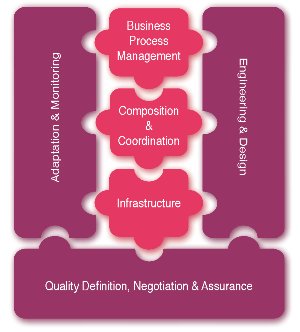
\includegraphics[width=.5\textwidth]{part1/pics/scube-overview.png}
  \caption{S-Cube Research Framework}
  \label{fig:scube-overview}
%	\vspace{0.2cm}  
\end{wrapfigure}
S-Cube~\footnote{http://www.s-cube-network.eu/} est un réseau d'excellence Européen en Logiciels, Services et Systèmes. Ce réseau d'excellence a pour ambition de faire de la recherche Européenne le leader de la révolution des services logiciels. En connectant la recherche à l'industrie, et en unifiant des recherches multidisciplinaires, S-Cube cherche à développer des méthodes d'ingénierie des services, agiles et globales, et spécifier les principes et techniques d'adaptation des services.\\
Ce réseau d'excellence a été financé par le programme de recherche Européen (FP7) 'Coordination', sous le thème des Technologies de la Communication et de l'Information (ICT). En plus d'offrir un fort support pour les collaboration et des opportunités de mobilité entre les instituts de recherches Européens, S-Cube a financé plusieurs thèses de doctorat pour les différentes couches de la "BigPicture" présentée en figure~\ref{fig:scube-overview}\\

L'excellence de l'équipe TRISKELL, dans laquelle cette thèse a été réalisée, réside en son savoir-faire pour faciliter le développement, et améliorer les méthodes de fabrication des logiciels, notamment par l'utilisation de modèles, de composants, de services et de techniques avancées de validation. Leader dans son domaine, l'équipe TRISKELL est impliquée dans le réseau S-Cube, qui finança cette thèse. Ainsi, les recherches qui ont menées aux résultats présentés dans cette thèse ont été financées par le septième programme de recherche Européen (FP7/2007-2013) sous l'agrément 215483 (S-Cube).


\subsection{Contribution}


La contribution de cette thèse s'inscrit dans les travaux du groupe de travail 1.2: {\it Adaptation and Monitoring Principles, Techniques and Methodologies for Service-based Systems} de l'activité de recherche collaborative(JRA) 1 : {\it Engineering and Adaptation Methodologies for Service-based Systems}\\

L'objectif général du JRA1 est de "concevoir un ensemble de principes intégrés, de techniques et de méthodologies pour la conception, l'adaptation et la surveillance d'applications hybrides basées sur les services, tout en garantissant la qualité du système de bout en bout, et sa conformité au contrat de service", d'après la description du travail d'S-Cube\footnote{DoW Amendment 4, December 6th, 2010}.\\
La contribution de cette thèse contient un modèle de composant qui: implique de nouvelles méthodes et techniques d'ingénierie, permet l'adaptation d'applications basées sur des services, et offre des moyens de réaliser des vérifications de al conception au déploiement pour assurer la qualité de service.\\

Plus précisément, la contribution de cette thèse d'inscrit dans le groupe de travaille JRA-1.2, qui cherche à définir de nouveaux principes et techniques pour l'adaptation et la surveillance d'applications orientées services, globalement sur l'ensemble des couches. Si \enti{} ne s'intéresse pas à priori aux problématiques de surveillance, il permet de résoudre les questions d'adaptation.\\

Du point de vue d'S-Cube, \enti{} pourrait être considéré pour participer à l'adaptation des couches d'infrastructure ou de composition et coordination de services, couches présentés sur la figure~\ref{fig:scube-overview}. 


\selectlanguage{english}